\chapter{Случайные события.}


\section*{Введение}

Задачи, с которыми сталкивается человек в окружающем мире, сформулированы на естественном языке. Первым этапом решения задачи является формализация --- формулировка задачи
с помощью математических объектов некоторой формальной схемы. В теории вероятностей такой схемой является \textbf{вероятностное пространство} $\left ( \Omega, \Sigma, P \right )$,
в котором:
\begin{enumerate}
    \item $\Omega$ --- множество элементарных исходов,
    \item $\Sigma$ --- алгебра событий,
    \item $P$ --- вероятностная мера.
\end{enumerate}

\section*{Задача 18.1}

Игральная кость подбрасывается дважды. Наблюдаемый результат --- пара чисел, соответствующих числам очков, выпавших в первый и второй раз. События:
\begin{itemize}
    \item $A = \event{\text{оба раза выпало число очков кратное трём}}$,
    \item $B = \event{\text{ни разу не выпало число шесть}}$,
    \item $C = \event{\text{оба раза выпало число очков, большее трех}}$,
    \item $D = \event{\text{оба раза выпало одинаковое число очков}}$.
\end{itemize}
Необходимо построить множество элементарных исходов $\Omega$ и подмножества, соответствующие событиям $A$ -- $D$.

\subsection*{Решение:}

\begin{enumerate}
    \item
    Каждый элементарный исход можно представить парой чисел $(i, j)$, где $i$ обозначает количество очков, выпавших в первый раз, а $j$ --- во второй, тогда множество всех элементарных
    исходов:
    \begin{equation}
        \Omega = \set{(i, j) : i, j \in \set{1, 2, 3, 4, 5, 6}}.
    \end{equation}

    Множество всех элементарных исходов удобно представить в виде таблицы:
    \begin{center}
        \begin{tabular}{c|c|c|c|c|c|c|}
            $i$, $j$ & 1         & 2         & 3         & 4         & 5         & 6         \\
            \hline
            1        & $\bullet$ & $\bullet$ & $\bullet$ & $\bullet$ & $\bullet$ & $\bullet$ \\
            \hline
            2        & $\bullet$ & $\bullet$ & $\bullet$ & $\bullet$ & $\bullet$ & $\bullet$ \\
            \hline
            3        & $\bullet$ & $\bullet$ & $\bullet$ & $\bullet$ & $\bullet$ & $\bullet$ \\
            \hline
            4        & $\bullet$ & $\bullet$ & $\bullet$ & $\bullet$ & $\bullet$ & $\bullet$ \\
            \hline
            5        & $\bullet$ & $\bullet$ & $\bullet$ & $\bullet$ & $\bullet$ & $\bullet$ \\
            \hline
            6        & $\bullet$ & $\bullet$ & $\bullet$ & $\bullet$ & $\bullet$ & $\bullet$ \\
            \hline
        \end{tabular}
    \end{center}

    \item
    Событие $A$ состоит из следующих элементарных исходов:
    \begin{equation}
        A = \set{(3,3), (3,6), (6,3), (6,6)} .
    \end{equation}
    В виде таблицы:
    \begin{center}
        \begin{tabular}{c|c|c|c|c|c|c|}
            $i$, $j$ & 1 & 2 & 3         & 4 & 5 & 6         \\
            \hline
            1        &   &   &           &   &   &           \\
            \hline
            2        &   &   &           &   &   &           \\
            \hline
            3        &   &   & $\bullet$ &   &   & $\bullet$ \\
            \hline
            4        &   &   &           &   &   &           \\
            \hline
            5        &   &   &           &   &   &           \\
            \hline
            6        &   &   & $\bullet$ &   &   & $\bullet$ \\
            \hline
        \end{tabular}
    \end{center}

    \item
    Событие $B$ состоит из следующих элементарных исходов:
    \begin{multline}
        B = \left \{ (1,1), (1,2), (1,3), (1,4), (1,5), \right . \\
        (2,1), (2,2), (2,3), (2,4), (2,5), \\
        (3,1), (3,2), (3,3), (3,4), (3,5), \\
        (4,1), (4,2), (4,3), (4,4), (4,5), \\
        \left . (5,1), (5,2), (5,3), (5,4), (5,5) \right \} .
    \end{multline}
    В виде таблицы:
    \begin{center}
        \begin{tabular}{c|c|c|c|c|c|c|}
            $i$, $j$ & 1         & 2         & 3         & 4         & 5         & 6 \\
            \hline
            1        & $\bullet$ & $\bullet$ & $\bullet$ & $\bullet$ & $\bullet$ &   \\
            \hline
            2        & $\bullet$ & $\bullet$ & $\bullet$ & $\bullet$ & $\bullet$ &   \\
            \hline
            3        & $\bullet$ & $\bullet$ & $\bullet$ & $\bullet$ & $\bullet$ &   \\
            \hline
            4        & $\bullet$ & $\bullet$ & $\bullet$ & $\bullet$ & $\bullet$ &   \\
            \hline
            5        & $\bullet$ & $\bullet$ & $\bullet$ & $\bullet$ & $\bullet$ &   \\
            \hline
            6        &           &           &           &           &           &   \\
            \hline
        \end{tabular}
    \end{center}

    \item
    Событие $C$ состоит из следующих элементарных исходов:
    \begin{equation}
        C = \set{(4,4), (4,5), (4,6), (5,4), (5,5), (5,6), (6,4), (6,5), (6,6)} .
    \end{equation}
    В виде таблицы:
    \begin{center}
        \begin{tabular}{c|c|c|c|c|c|c|}
            $i$, $j$ & 1 & 2 & 3 & 4         & 5         & 6         \\
            \hline
            1        &   &   &   &           &           &           \\
            \hline
            2        &   &   &   &           &           &           \\
            \hline
            3        &   &   &   &           &           &           \\
            \hline
            4        &   &   &   & $\bullet$ & $\bullet$ & $\bullet$ \\
            \hline
            5        &   &   &   & $\bullet$ & $\bullet$ & $\bullet$ \\
            \hline
            6        &   &   &   & $\bullet$ & $\bullet$ & $\bullet$ \\
            \hline
        \end{tabular}
    \end{center}

    \item
    Событие $D$ состоит из следующих элементарных исходов:
    \begin{equation}
        D = \set{(1,1), (2,2), (3,3), (4,4), (5,5), (6,6)} .
    \end{equation}
    В виде таблицы:
    \begin{center}
        \begin{tabular}{c|c|c|c|c|c|c|}
            $i$, $j$ & 1         & 2         & 3         & 4         & 5         & 6         \\
            \hline
            1        & $\bullet$ &           &           &           &           &           \\
            \hline
            2        &           & $\bullet$ &           &           &           &           \\
            \hline
            3        &           &           & $\bullet$ &           &           &           \\
            \hline
            4        &           &           &           & $\bullet$ &           &           \\
            \hline
            5        &           &           &           &           & $\bullet$ &           \\
            \hline
            6        &           &           &           &           &           & $\bullet$ \\
            \hline
        \end{tabular}
    \end{center}
\end{enumerate}

\subsection*{Ответ:}
\begin{enumerate}
    \item $\Omega = \set{(i, j) : i, j \in \set{1, 2, 3, 4, 5, 6}}$,
    \item $A = \set{(i, j) : i, j \in \set{3, 6}}$,
    \item $B = \set{(i, j) : i, j \in \set{1, 2, 3, 4, 5}}$,
    \item $C = \set{(i, j) : i, j \in \set{4, 5, 6}}$,
    \item $D = \set{(i, i) : i \in \set{1, 2, 3, 4, 5, 6}}$.
\end{enumerate}

\section*{Задача 18.3}

Монета подбрасывается до первого появления герба. Наблюдаемый результат --- общее число подбрасываний. События:
\begin{enumerate}
    \item $A = \event{\text{герб выпал при третьем подбрасывании}}$,
    \item $B = \event{\text{герб выпал не ранее, чем при третьем подбрасывании}}$.
\end{enumerate}
Построить множество элементарных исходов $\Omega$ и подмножества, соответствующие событиям $A$ и $B$.

\subsection*{Решение:}

Элементарные исходы представим в виде конечного набора решек ("Р"), которые заканчиваются гербом ("Г"):
\begin{align*}
    \omega_1 = & \left ( \text{Г} \right ) , \\
    \omega_2 = & \left ( \text{Р}, \text{Г} \right ) , \\
    \omega_3 = & \left ( \text{Р}, \text{Р}, \text{Г} \right ) , \\
    \omega_4 = & \left ( \text{Р}, \text{Р}, \text{Р}, \text{Г} \right ) , \\
    & \dots \\
    \omega_n = & \left ( \overbrace{\text{Р}, \dots, \text{Р}}^{n-1}, \text{Г} \right ), \\
    & \dots
\end{align*}
Множество всех элеметарных исходов $\Omega = \set{\omega_1, \omega_2, \omega_3, \omega_4, \dots }$. В данном случае множество $\Omega$ является счетным.

Событие $A = \set{\omega_3}$, событие $B = \set{\omega_i : 3 \le i}$.

\subsection*{Ответ:}
Элементарный исход $\omega_n$ обозначает выпадение герба на $n$-ом подбрасывании.
\begin{enumerate}
    \item $\Omega = \set{\omega_n: n \in \mathbb{N}}$,
    \item $A = \set{\omega_3}$,
    \item $B = \set{\omega_i: 3 \le i}$.
\end{enumerate}


\section*{Задача 18.5}

Производится стрельба по плоской прямоугольной мишени: $-2 \le x \le 2$, $-1 \le y \le 1$. Наблюдаемый результат --- координаты точки попадания в декартовой системе координат.
По условиям стрельбы непопадание в указанный прямоугольник исключено. События:
\begin{enumerate}
    \item $A = \event{\text{абсцисса точки попадания не меньше ординаты}}$,
    \item $B = \event{\text{произведение координат точки неотрицательно}}$,
    \item $C = \event{\text{сумма абсолютных величин координат точки превышает единицу}}$.
\end{enumerate}
Построить множество элементарных исходов $\Omega$ и подмножества, соответствующие событиям. Выявить пары совместных событий.

\subsection*{Решение:}

Элементарным исходом является пара координат $\left ( x, y \right )$, где $-2 \le x \le 2$ и $-1 \le y \le 1$. Множество элементарных исходов $\Omega$ --- прямоугольник:
\begin{equation}
    \Omega = \set{(x, y): -2 \le x \le 2, -1 \le y \le 1}.
\end{equation}

\begin{figure}[h]
    \centering
    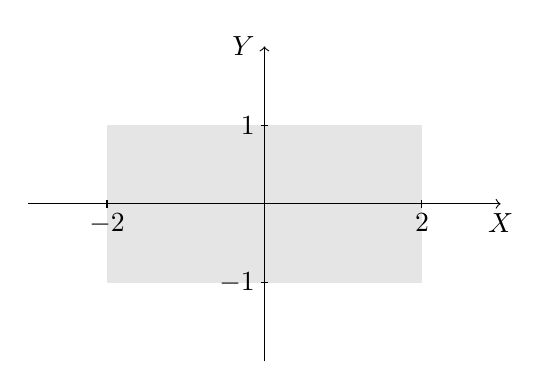
\begin{tikzpicture}
        % множество
        \path [fill=gray!20] ( -2, -1 ) rectangle ( 2, 1 );

        % оси
        \draw [->] ( -3, 0 ) -- ( 3, 0 ) node [below] at ( 3, 0 ) {$X$};
        \draw [->] ( 0, -2 ) -- ( 0, 2 ) node [left] at ( 0, 2 ) {$Y$};

        % отметки
        \draw ( 2, -0.05 ) -- ( 2, 0.05 ) node [below] at ( 2, 0 ) {$2$};
        \draw ( -2, -0.05 ) -- ( -2, 0.05 ) node [below] at ( -2, 0 ) {$-2$};
        \draw ( -0.05, 1 ) -- ( 0.05, 1 ) node [left] at ( 0, 1 ) {$1$};
        \draw ( -0.05, -1 ) -- ( 0.05, -1 ) node [left] at ( 0, -1 ) {$-1$};
    \end{tikzpicture}
    \caption{Множество элементаных исходов $\Omega$.}
\end{figure}

События:
\begin{enumerate}
    \item $A = \set{(x, y): x \ge y}$,
    \item $B = \set{(x, y): x \cdot y \ge 0}$,
    \item $C = \set{(x, y): \modulus{x} + \modulus{y} > 1}$.
\end{enumerate}

Совместными являются события, которые могут наступить одновременно, то есть события, у которых есть общие элементарные исходы. Пары совместных событий: $A$ и $B$, $A$ и $C$,
$B$ и $C$.

\begin{figure}[h]
    \centering
    \begin{subfigure}{0.3\textwidth}
        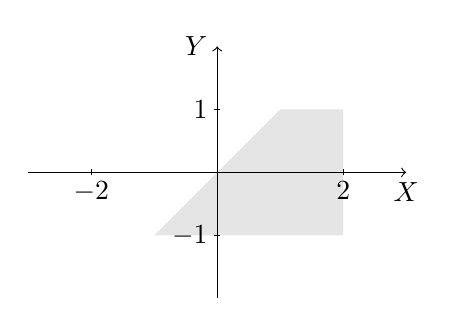
\begin{tikzpicture}[scale=0.8]
            % множество
            \path [fill=gray!20] ( -1, -1 ) -- ( 1, 1 ) -- ( 2, 1 ) -- ( 2, -1 ) -- ( -1, -1 );
            % оси
            \draw [->] ( -3, 0 ) -- ( 3, 0 ) node [below] at ( 3, 0 ) {$X$};
            \draw [->] ( 0, -2 ) -- ( 0, 2 ) node [left] at ( 0, 2 ) {$Y$};

            % отметки
            \draw ( 2, -0.05 ) -- ( 2, 0.05 ) node [below] at ( 2, 0 ) {$2$};
            \draw ( -2, -0.05 ) -- ( -2, 0.05 ) node [below] at ( -2, 0 ) {$-2$};
            \draw ( -0.05, 1 ) -- ( 0.05, 1 ) node [left] at ( 0, 1 ) {$1$};
            \draw ( -0.05, -1 ) -- ( 0.05, -1 ) node [left] at ( 0, -1 ) {$-1$};
        \end{tikzpicture}
        \caption{Событие $A$}
    \end{subfigure}
    \hfill
    \begin{subfigure}{0.3\textwidth}
        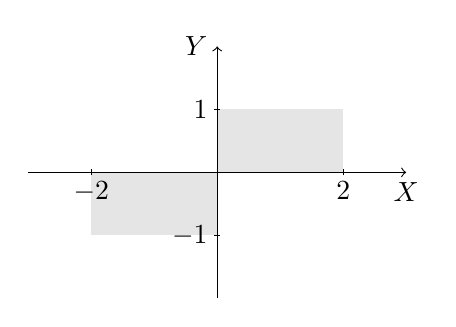
\begin{tikzpicture}[scale=0.8]
            % множество
            \path [fill=gray!20] ( -2, -1 ) rectangle ( 0, 0 );
            \path [fill=gray!20] ( 0, 0 ) rectangle ( 2, 1 );

            % оси
            \draw [->] ( -3, 0 ) -- ( 3, 0 ) node [below] at ( 3, 0 ) {$X$};
            \draw [->] ( 0, -2 ) -- ( 0, 2 ) node [left] at ( 0, 2 ) {$Y$};

            % отметки
            \draw ( 2, -0.05 ) -- ( 2, 0.05 ) node [below] at ( 2, 0 ) {$2$};
            \draw ( -2, -0.05 ) -- ( -2, 0.05 ) node [below] at ( -2, 0 ) {$-2$};
            \draw ( -0.05, 1 ) -- ( 0.05, 1 ) node [left] at ( 0, 1 ) {$1$};
            \draw ( -0.05, -1 ) -- ( 0.05, -1 ) node [left] at ( 0, -1 ) {$-1$};
        \end{tikzpicture}
        \caption{Событие $B$}
    \end{subfigure}
    \hfill
    \begin{subfigure}{0.3\textwidth}
        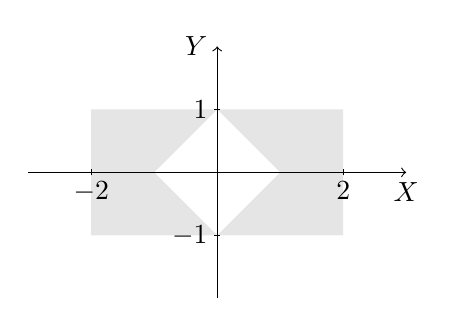
\begin{tikzpicture}[scale=0.8]
            % множество
            \path [fill=gray!20] ( 0, 1 ) -- ( 2, 1 ) -- ( 2, 0 ) -- ( 1, 0 );
            \path [fill=gray!20] ( 0, 1 ) -- ( -2, 1 ) -- ( -2, 0 ) -- ( -1, 0 );
            \path [fill=gray!20] ( 0, -1 ) -- ( 2, -1 ) -- ( 2, 0 ) -- ( 1, 0 );
            \path [fill=gray!20] ( 0, -1 ) -- ( -2, -1 ) -- ( -2, 0 ) -- ( -1, 0 );

            % оси
            \draw [->] ( -3, 0 ) -- ( 3, 0 ) node [below] at ( 3, 0 ) {$X$};
            \draw [->] ( 0, -2 ) -- ( 0, 2 ) node [left] at ( 0, 2 ) {$Y$};

            % отметки
            \draw ( 2, -0.05 ) -- ( 2, 0.05 ) node [below] at ( 2, 0 ) {$2$};
            \draw ( -2, -0.05 ) -- ( -2, 0.05 ) node [below] at ( -2, 0 ) {$-2$};
            \draw ( -0.05, 1 ) -- ( 0.05, 1 ) node [left] at ( 0, 1 ) {$1$};
            \draw ( -0.05, -1 ) -- ( 0.05, -1 ) node [left] at ( 0, -1 ) {$-1$};
        \end{tikzpicture}
        \caption{Событие $C$}
    \end{subfigure}
    \caption{События $A$, $B$, $C$.}
\end{figure}

\subsection*{Ответ:}
\begin{enumerate}
    \item Множество всех элементарных исходов $\Omega = \set{(x, y): -2 \le x \le 2, -1 \le y \le 1}$.
    \item $A = \set{(x, y): x \ge y}$.
    \item $B = \set{(x, y): x \cdot y \ge 0}$.
    \item $C = \set{(x, y): \modulus{x} + \modulus{y} > 1}$.
    \item Пары совместных событий: $A$ и $B$, $A$ и $C$, $B$ и $C$.
\end{enumerate}


\section*{Задача 18.16}

Показать справедливость равенства: $A - B = A \overline{B}$.

\subsection*{Решение:}

\begin{enumerate}
    \item Если $A - B \neq \emptyset$:
    \begin{equation}
        \omega \in A - B
        \Leftrightarrow
        \left \{
        \begin{array}{l}
            \omega \in A \\
            \omega \notin B
        \end{array}
        \right .
        \Leftrightarrow
        \left \{
        \begin{array}{l}
            \omega \in A \\
            \omega \in \overline{B}
        \end{array}
        \right .
        \Leftrightarrow
        \omega \in A \overline{B} .
    \end{equation}

    \item Если $A - B = \emptyset$:
    \begin{equation}
        A - B = \emptyset
        \Leftrightarrow
        \omega \in A \rightarrow \omega \in B
        \Leftrightarrow
        \omega \in A \rightarrow \omega \notin \overline{B}
        \Leftrightarrow
        A \overline{B} = \emptyset .
    \end{equation}
\end{enumerate}


\section*{Задача 18.23}

Показать справедливость равенства: $\left ( A + B \right ) \left ( A + \overline{B} \right ) = A$.

\subsection*{Решение:}

\begin{multline}
    \left ( A + B \right ) \left ( A + \overline{B} \right )
    = A \left ( A + \overline{B} \right ) + B \left ( A + \overline{B} \right )
    = A A + A \overline{B} + B A + B \overline{B} = \\
    %
    = A + A \overline{B} + B A + \emptyset
    = A + A \overline{B} + A B
    = A + A \left ( \overline{B} + B \right )
    = A + A \Omega = \\
    %
    = A + A
    = A
    .
\end{multline}

\section*{Задача 18.35}

Пусть $A$, $B$ и $C$ --- наблюдаемые события. Выразить с помощью $A$, $B$ и $C$ события:
\begin{enumerate}
    \item $E = \event{\text{из трех событий } A, B, C \text{ произойдет ровно одно}}$,
    \item $F = \event{\text{из трех событий } A, B, C \text{ произойдет ровно два}}$.
\end{enumerate}

\subsection*{Решение:}

\begin{enumerate}
    \item
    Подумаем, когда происходит только одно событие:
    \begin{enumerate}
        \item происходит $A$, но не происходят ни $B$, ни $C$:
        \item не происходит $A$, зато происходит $B$, но не происходит $C$,
        \item не происходит ни $A$, ни $B$, но происходит $C$.
    \end{enumerate}

    Попробуем записать через элементарные исходы:
    \begin{enumerate}
        \item $\omega \in A, \omega \notin B, \omega \notin C \Leftrightarrow \omega \in A, \omega \in \overline{B}, \omega \in \overline{C} \Leftrightarrow \omega \in A \cdot \overline{B} \cdot \overline{C}$
        \item $\omega \notin A, \omega \in B, \omega \notin C \Leftrightarrow \omega \in \overline{A}, \omega \in B, \omega \in \overline{C} \Leftrightarrow \omega \in \overline{A} \cdot B \cdot \overline{C}$
        \item $\omega \notin A, \omega \notin B, \omega \in C \Leftrightarrow \omega \in \overline{A}, \omega \in \overline{B}, \omega \in C \Leftrightarrow \omega \in \overline{A} \cdot \overline{B} \cdot C$
    \end{enumerate}

    В итоге приходим к выражению:
    \begin{equation}
        E = A \cdot \overline{B} \cdot \overline{C} + \overline{A} \cdot B \cdot \overline{C} + \overline{A} \cdot \overline{B} \cdot C .
    \end{equation}

    \item
    Аналогично
    \begin{equation}
        F = A \cdot B \cdot \overline{C} + A \cdot \overline{B} \cdot C + \overline{A} \cdot B \cdot C .
    \end{equation}
\end{enumerate}

\subsection*{Ответ:}
\begin{enumerate}
    \item $E = A \cdot \overline{B} \cdot \overline{C} + \overline{A} \cdot B \cdot \overline{C} + \overline{A} \cdot \overline{B} \cdot C$,
    \item $F = A \cdot B \cdot \overline{C} + A \cdot \overline{B} \cdot C + \overline{A} \cdot B \cdot C$.
\end{enumerate}


\section*{Задача 18.36}

Пусть $A$, $B$ и $C$ --- наблюдаемые события. Выразить с помощью $A$, $B$ и $C$ события:
\begin{enumerate}
    \item $E = \event{\text{из трех событий } A, B, C \text{ произойдет хотя бы одно}}$,
    \item $F = \event{\text{из трех событий } A, B, C \text{ произойдет не меньше двух}}$.
\end{enumerate}

\subsection*{Решение:}

\begin{enumerate}
    \item
    Заметим, что событие "произойдет хотя бы одно событие"{} означает, что "произойдет ровно одно событие"{}, или "произойдут ровно два события"{} или "произойдут все три события"{}.
    Рассуждая аналогично задаче 35, для события $E$ можно получить следующее выражение:
    \begin{align}
        E & = A \cdot \overline{B} \cdot \overline{C} + \overline{A} \cdot B \cdot \overline{C} + \overline{A} \cdot \overline{B} \cdot C + \\
        & + A \cdot B \cdot \overline{C} + A \cdot \overline{B} \cdot C + \overline{A} \cdot B \cdot C + \\
        & + A \cdot B \cdot C
    \end{align}
    Это довольно длинное выражение, но его можно заменить более коротким, если заметить, что дополнительное событие "не произойдет ни одного события"{} имеет простое выражение:
    \[
        \overline{E} = \overline{A} \cdot \overline{B} \cdot \overline{C}
    \]
    и поскольку:
    \begin{gather}
        E + \overline{E} = \Omega, \\
        E = \Omega - \overline{E}, \\
        E = \Omega - \overline{A} \cdot \overline{B} \cdot \overline{C}
    \end{gather}

    \item
    Аналогично, событие "произойдет не менее двух событий"{} означает, что "произойдут ровно два события"{} или "произойдут все три события"{}:
    \begin{align}
        F & = A \cdot B \cdot \overline{C} + A \cdot \overline{B} \cdot C + \overline{A} \cdot B \cdot C + \\
        & + A \cdot B \cdot C .
    \end{align}
    А через дополнительное событие:
    \begin{align}
        F & = \Omega - \left ( A \cdot \overline{B} \cdot \overline{C} + \overline{A} \cdot B \cdot \overline{C} + \overline{A} \cdot \overline{B} \cdot C + \overline{A} \cdot \overline{B} \cdot \overline{C} \right ) .
    \end{align}
\end{enumerate}

\subsection*{Ответ:}
\begin{enumerate}
    \item $E = \Omega - \overline{A} \cdot \overline{B} \cdot \overline{C}$,
    \item $F = A \cdot B \cdot \overline{C} + A \cdot \overline{B} \cdot C + \overline{A} \cdot B \cdot C + A \cdot B \cdot C .$
\end{enumerate}

\section*{Задача 18.39}

Электрическая цепь составлена по схеме, приведенной на рисунке. \\
\begin{figure}[h]
    \centering
    \begin{tikzpicture}
        % вход
        \draw ( -0.5, 0.5 ) -- ( 0, 0.5 );

        % 1
        \draw ( 0, 0 ) -- ( 0, 1 ) -- ( 1, 1 ) -- ( 1, 0 ) -- ( 0, 0 ) node at ( 0.5, 0.5 ) {$1$};
        % 1-[2,3]
        \draw ( 1, 0.5 ) -- ( 2, 0.5 ) -- ( 2, 1.5 ) -- ( 3, 1.5 );
        \draw ( 2, 0.5 ) -- ( 2, -0.5 ) -- ( 3, -0.5 );

        % 2
        \draw ( 3, 2 ) -- ( 4, 2 ) -- ( 4, 1 ) -- ( 3, 1 ) -- ( 3, 2 ) node at ( 3.5, 1.5 ) {$2$};
        % 3
        \draw ( 3, 0 ) -- ( 4, 0 ) -- ( 4, -1 ) -- ( 3, -1 ) -- ( 3, 0 ) node at ( 3.5, -0.5 ) {$3$};

        % [2,3]-4
        \draw ( 4, 1.5 ) -- ( 5, 1.5 ) -- ( 5, 0.5 ) -- ( 6, 0.5 );
        \draw ( 4, -0.5 ) -- ( 5, -0.5 ) -- ( 5, 0.5 );

        % 4
        \draw ( 6, 1 ) -- ( 7, 1 ) -- ( 7, 0 ) -- ( 6, 0 ) -- ( 6, 1 ) node at ( 6.5, 0.5 ) {$4$};

        % выход
        \draw ( 7, 0.5 ) -- ( 7.5, 0.5 );
    \end{tikzpicture}
    \caption{Электрическая цепь.}
\end{figure}

Событие $A_k = \event{\text{элемент с номером } k \text{ вышел из строя}}$, $k = 1, 2, 3, 4$. Событие
$B = \event{\text{разрыв цепи}}$. Выразить событие $B$ в алгебре событий $A_1$, $A_2$, $A_3$, $A_4$.

\subsection*{Решение:}

В схеме элемент 1, группа 2-3 и элемент 4 расположены последовательно, поэтому разрыв цепи произойдет, если вышел из строя элемент 1 или группа элементов 2-3 или
элемент 4:
\begin{equation}
    B = A_1 + B_{2-3} + A_4 ,
\end{equation}
где $B_{2-3}$ --- событие "вышла из строя группа элементов 2-3". В группе элементов "2-3"{} элементы соединены параллельно, поэтому отказ группы происходит, если отказывают
одновременно и элемент 2, и элемент 3:
\begin{equation}
    B_{2-3} = A_2 \cdot A_3.
\end{equation}
Подставляя выражение для $B_{2-3}$ получим:
\begin{equation}
    B = A_1 + A_2 \cdot A_3 + A_4.
\end{equation}

\subsection*{Ответ:}
$B = A_1 + A_2 \cdot A_3 + A_4$.

\section*{Задача 18.42.а)}

Произведено три выстрела из орудия по цели. Событие $A_k = \event{\text{попадание при } k \text{-ом выстреле}}$, $k=1,2,3$. Выяснить состав множества $\Omega$, выразив
каждый элементарный исход $\omega_i$ через события $A_k$.

\subsection*{Решение:}

Множество $\Omega$ состоит из следующих элементарных исходов:

\begin{center}
    \begin{tabular}{|c|c|c|c|c|}
        \hline
        Исход    & Выстрел 1 & Выстрел 2 & Выстрел 3 & Представление                                              \\
        \hline
        $\omega_0$ &           &           &           & $\overline{A_1} \cdot \overline{A_2} \cdot \overline{A_3}$ \\
        \hline
        $\omega_1$ &           & $\bullet$ &           & $\overline{A_1} \cdot A_2 \cdot \overline{A_3}$            \\
        \hline
        $\omega_2$ &           &           & $\bullet$ & $\overline{A_1} \cdot \overline{A_2} \cdot A_3$            \\
        \hline
        $\omega_3$ &           & $\bullet$ & $\bullet$ & $\overline{A_1} \cdot A_2 \cdot A_3$                       \\
        \hline
        $\omega_4$ & $\bullet$ &           &           & $A_1 \cdot \overline{A_2} \cdot \overline{A_3}$            \\
        \hline
        $\omega_5$ & $\bullet$ & $\bullet$ &           & $A_1 \cdot A_2 \cdot \overline{A_3}$                       \\
        \hline
        $\omega_6$ & $\bullet$ &           & $\bullet$ & $A_1 \cdot \overline{A_2} \cdot A_3$                       \\
        \hline
        $\omega_7$ & $\bullet$ & $\bullet$ & $\bullet$ & $A_1 \cdot A_2 \cdot A_3$                                  \\
        \hline
    \end{tabular}
\end{center}

\section*{Задача 18.42 (полная группа)}

Показать, что набор событий $B_k$, где $k$ --- количество попаданий, образуют полную группу событий.

\subsection*{Решение:}

Выразим события $B_k$ через элементарные исходы:
\begin{align}
    B_0 & = \set{ \omega_0 }, \\
    B_1 & = \set{ \omega_1, \omega_2, \omega_4 }, \\
    B_2 & = \set{ \omega_3, \omega_5, \omega_6 }, \\
    B_3 & = \set{ \omega_7 }.
\end{align}

Легко видеть, что любые два события $B_i$ и $B_j$ не пересекаются:
\[
    B_i \cap B_j = \emptyset
\]
и при этом их объединение образует множество всех элементарных исходов:
\[
    B_0 \cup B_1 \cup B_2 \cup B_3 = \bigcup_{i=0}^7 \omega_i = \Omega .
\]

\section*{Задачи для самостоятельного решения}

Из раздела 18 сборника задач Ефимова и Поспелова.
\begin{enumerate}
    \item На занятии: 2, 24, 40.
    \item Дома: 4, 6, 13, 14, 19, 29, 42б, 43.
\end{enumerate}